\documentclass[../main.tex]{subfiles}
\begin{document}
    \chapter{Research Method}\label{chap:research_method}
    %This section will contain:
    %TODO: Explain the used method. %TODO research method
    %TODO: Hypothese/research questions %TODO research question
    $<<$ Introduction of this chapter $>>$
    \\
    Maybe add a section here explaining all the steps taken in this research... to be added later.
    It is not very likely to keep Types as first chapter.
    \blindtext %todo remove blind text
    
    \section{Types}
    Explain here what I mean with a type...
    
    \begin{rascal}
\CAT{Keyword}{module} lang::php::m3::TypeSymbol

\CAT{Keyword}{data} TypeSymbol
  = any()
  | array(\CAT{Keyword}{set}{}[TypeSymbol] itemTypes)
  | \textbackslash{}bool()
  | class(\CAT{Keyword}{loc} decl)
  | float()
  | \textbackslash{}int()
  | object()
  | resource()
  | \textbackslash{}null()
  | string()
  | unset()
  ; 
    \end{rascal}
    
    \subsection{PHP types}
    PHP has a similar class inheritance structure and interface implementation as Java.
    The main difference is that in PHP all class are \texttt{public} and that inner classes are not allowed in PHP. 
    \\
    The basis types in PHP are integers, floats (similar to doubles and reals), booleans, strings, arrays, resources and null.
    When variables are initialised without a values, they are null. The recourse type is a special one which is not important for this research.
 
    \subsection{Subtypes}
    
    Explain something about subtypes here.

    \blindtext %todo remove blind text
    
    \begin{figure}[H]
        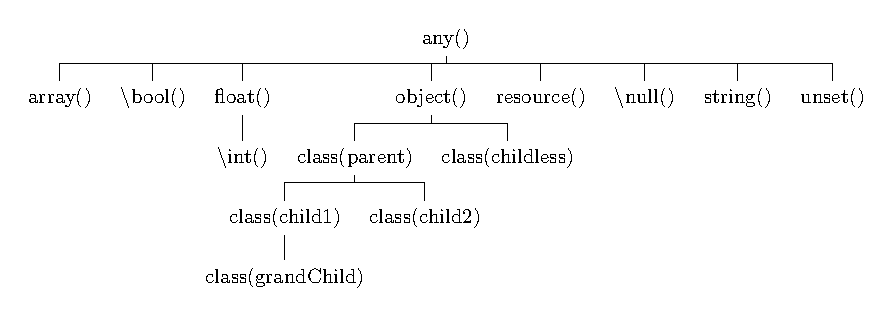
\includegraphics{Diagrams/Subtypes.pdf}
        \caption{Subtype hierarchy}
        \label{fig:subtypes}
    \end{figure}
 
    % show two images next to eachother
    \begin{wrapfigure}{r}{0.5\textwidth}
    \begin{subfigure}{.24\textwidth}
      \begin{center}
      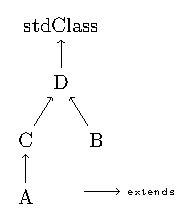
\includegraphics[scale=1.25]{Diagrams/Inheritance_example.pdf}
      \caption{Inheritance relation}
      \label{fig:subtype}
      \end{center}
    \end{subfigure}
    \begin{subfigure}{.24\textwidth}
      \begin{center}
      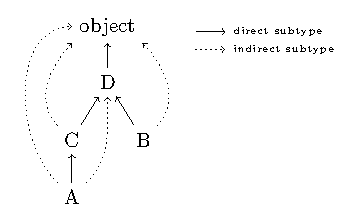
\includegraphics[scale=1.25]{Diagrams/Subtypes_example.pdf}
      \caption{Subtype relation}
      \label{subtype_tc}
      \end{center}
    \end{subfigure}
    \lstinputlisting[xleftmargin=20pt,xrightmargin=20pt,aboveskip=20pt,language=PHP,label=inheritance,caption=Inheritance in PHP]{src/php/inheritance.php}
    \caption{Relation of subtypes among classes}
    \label{fig:subtypes}
    \end{wrapfigure}

    The subtype relation of class inheritance is a \gls{reflexive transitive closure} relation.
    A class extension of \underline{\texttt{class A}} on \underline{\texttt{class C}} will define \underline{\texttt{class A}} as a subtype of \underline{\texttt{class C}} in our analysis, as you can see in figure \ref{fig:subtypes}.
    If a class does not extend another class, it will implicitly extend the \gls{stdClass} class.
    You can see that this happens with \underline{\texttt{class D}} in the example.
    The \underline{\texttt{stdClass}} is represented as the type \underline{\texttt{object()}} in our analysis.
    \\
    The basic PHP types also contain a subtype relation.
    Integers are subtypes of floats.
    
    
    \section{Fact extraction}
    Here I need to explain that I will extract types and subtypes and constraints from the source code an how I do that.
    
    \subsection{Type extraction}
    In order to define the subtype relations in class extensions, we will need to declare all existing class types.
    We can do this in rascal like is done in the example below:
    \begin{rascal}
\CAT{Keyword}{visit} (system) \{{}
    \CAT{Keyword}{case} c:class(\_{}, \_{}, \_{}, \_{}, \_{}): types += class(c@decl);
\}{}
    \end{rascal}
    Once all types are defined, we can add the subtype relation. We will need to have the subtype of \texttt{int()} and \texttt{float()} and the class extensions.
    You can see that in the code below:
    \begin{rascal}
\CAT{Keyword}{public} \CAT{Keyword}{rel}{}[TypeSymbol, TypeSymbol] getSubTypes(M3 m3, System system) 
\{{}
    \CAT{Keyword}{rel}{}[TypeSymbol, TypeSymbol] subtypes
        \CAT{Comment}{// add int() as subtype of float()}
        = \{{} \textless{}\textbackslash{}int(), float()\textgreater{} \}{} 
        \CAT{Comment}{// use the extends relation from M3}
        + \{{} \textless{}class(c), class(e)\textgreater{} | \textless{}c,e\textgreater{} \textless{}- m3@extends \}{}
        \CAT{Comment}{// add subtype of object for all classes which do not extends a class}
        + \{{} \textless{}class(c@decl), object()\textgreater{} | l \textless{}- system, /c:class(n,\_{},noName(),\_{},\_{}) \textless{}- system{}[l] \}{};
        
    \CAT{Comment}{// compute reflexive transitive closure and return the result }
    \CAT{Keyword}{return} subtypes*;        
\}{}
    \end{rascal}
    
    \subsection{Constraint extraction}
       
    Introduction is needed here... for now I will just list the types that I have found.
    Maybe this needs to be moved to a different chapter.
    \\
    This is a list of items which are not supported yet:

    \begin{itemize}
        \item Assign statements:
        \begin{itemize}
            \item Ref assign :: $\$a \; = \; \&\$b$
            \item List assign :: $list(\$a, \$b) = array("one", "two");$
        \end{itemize}
        
        \item References (in PHP they are symbol table aliases)
        \begin{itemize}
            \item on expression assignments :: $\$a \; = \; \&\$b$
            \item on functions :: function $\&f()$ $\{ \dots \}$
            \item on parameters :: function $f(\$a)$ $\{ \dots \}$             
        \end{itemize}

        \item Variable structures:
        \begin{itemize}
            \item Variable variables :: $\$\$a;$
            \item \sout{Variable class instantiation} :: $new \; \$a;$
            \item \sout{Variable method or function calls} :: $\$a();$
        \end{itemize}
        
        \item Method or function parameters (including type hints)
        
        \item Casts of expressions
        
        
    \end{itemize}

    \hrulefill
    \\
    Note to myself ::
    \\
    type has field \\
    type has name \\
    type has method \\
    type has magic method \\
    
    \hrulefill
    
    \textbf{Legend} \\
    \begin{table}[H]
        \begin{tabular}{ r c l }
            $=$     & = & Equal to (type) \\
            $<:$    & = & Is subTypeOf \\
            $E_k$   & = & Some expression\\
            $[E_k]$ & = & Type of some expression \\
            $f$     & = & Some function
        \end{tabular}
        \caption{Constraint legend}
        \label{table:constraintLegend}
    \end{table}
    
    \subsubsection{Expressions}
    Normal assignment:
    \begin{prooftree}
        \AxiomC{$E_1 = E_2$}
        \UnaryInfC{$[E_2]<:[E_1]$}
    \end{prooftree}
    \lstinputlisting[language=PHP,label=assignment1,caption=Assignment]{src/php/assignment1.php}
    \hrulefill

    Ternary:
    \begin{prooftree}
        \AxiomC{$E_1 \; ? \; E_2 : E_3 $}
        \UnaryInfC{$[E_1?E_2:E_3] = [E_3] \lor [E_4]$}
    \end{prooftree}
    \lstinputlisting[language=PHP,label=ternary.php,caption=Ternary]{src/php/ternary.php}
    \hrulefill

    Assignments with operators (1)
    \begin{prooftree}
        \AxiomC{
        ($E_1$ $\&=$ $E_2$) $\lor$
        ($E_1$ $\vert=$ $E_2$) $\lor$
        $E_1$ \^{}= $E_2$) $\lor$
        ($E_1$ $<<=$ $E_2$) $\lor$
        ($E_1$ $>>=$ $E_2$) $\lor$
        ($E_1$ $\%=$ $E_2$)
        }
        \UnaryInfC{$[E_1] = int()$}
    \end{prooftree}
    \lstinputlisting[language=PHP,label=assignment2,caption=Assignments with operators resulting in ints]{src/php/assignment2.php}
    \hrulefill

    Assignments with operators (2):
    \begin{prooftree}
        \AxiomC{$E_1$ .= $E_2$}
        \UnaryInfC{$[E_1] = string()$}
    \end{prooftree}    
    \lstinputlisting[language=PHP,label=assignment3,caption=Assignments with string concat operator]{src/php/assignment3.php}    
    \hrulefill
    
    Assignments with operators (3):
    \begin{prooftree}
        \AxiomC{
        ($E_1$ $/= E_2$) $\lor$
        ($E_1 -= E_2$)
        }
        \UnaryInfC{$[E_1] = int()$}
    \end{prooftree}    
    \lstinputlisting[language=PHP,label=assignment4,caption=Assignments with operators]{src/php/assignment4.php}
    \hrulefill

    Assignment with operators (4):            
    \begin{prooftree}
        \AxiomC{
        ($E_1$ *= $E_2$) $\lor$
        ($E_1$ += $E_2$)
        }
        \UnaryInfC{$[E_1] <: int()$}
    \end{prooftree}    
    \lstinputlisting[language=PHP,label=assignment5,caption=Assignments with operators]{src/php/assignment5.php}
    \hrulefill

    Comparison operators:    
    \begin{prooftree}
        \AxiomC{
        ($E_1$ $==$ $E_2$) $\lor$
        ($E_1$ $===$ $E_2$) $\lor$
        ($E_1$ $!=$ $E_2$) $\lor$
        ($E_1$ $<>$ $E_2$) $\lor$
        ($E_1$ $!==$ $E_2$)
        $\subseteq E$
        }
        \UnaryInfC{$[E] = bool()$}
    \end{prooftree}    
    \begin{prooftree}
        \AxiomC{
        ($E_1$ $<$ $E_2$) $\lor$
        ($E_1$ $>$ $E_2$) $\lor$
        ($E_1$ $<=$ $E_2$) $\lor$
        ($E_1$ $>=$ $E_2$)
        $\subseteq E$
        }
        \UnaryInfC{$[E] = bool()$}
    \end{prooftree}    
    \lstinputlisting[language=PHP,label=comparisonOperators.php,caption=Comparison operators]{src/php/comparisonOperators.php}
    \hrulefill
    
    Array declaration:
    \begin{prooftree}
        \AxiomC{
        $E'$, where $E'$ is an array declaration
        }
        \UnaryInfC{$[E'] = array()$}
    \end{prooftree} 
    \lstinputlisting[language=PHP,label=array.php,caption=Array declaration]{src/php/array.php}
    \hrulefill

    Array value fetch:
    \begin{prooftree}
        \AxiomC{$E_1[E_2]$ $\land$ $E_1 == string()$, where $E_1$ is an array}
        \UnaryInfC{$[E_1[E_2]] = string()$}
    \end{prooftree} 
    \begin{prooftree}
        \AxiomC{$E_1[E_2]$ $\land$ $E_1 == array()$, where $E_1$ is an array}
        \UnaryInfC{$[E_1[E_2]] = mixed()$}
    \end{prooftree} 
    \begin{prooftree}
        \AxiomC{$E_1[E_2]$ $\land$ $(E_1 == string()$ $\lor$ $E_1 == array())$, where $E_1$ is an array}
        \UnaryInfC{$[E_1[E_2]] = null()$}
    \end{prooftree} 
    \lstinputlisting[language=PHP,label=array.php,caption=Array value fetch]{src/php/arrayAccess.php}
    \hrulefill
    
    \subsubsection{Casts}
    Casts:
    \begin{prooftree}
        \AxiomC{$(array)E_1$}
        \UnaryInfC{$[(cast)E_1] = array()$}
    \end{prooftree}
    \begin{prooftree}
        \AxiomC{$(bool)E_1$ $\lor$ $(boolean)E_1$}
        \UnaryInfC{$[(cast)E_1] = bool()$}
    \end{prooftree}
    \begin{prooftree}
        \AxiomC{$(float)E_1$ $\lor$ $(double)E_1$ $\lor$ $(real)E_1$}
        \UnaryInfC{$[(cast)E_1] = float()$}
    \end{prooftree}    
    \begin{prooftree}
        \AxiomC{$(int)E_1$ $\lor$ $(integer)E_1$}
        \UnaryInfC{$[(cast)E_1] = int()$}
    \end{prooftree}
    \begin{prooftree}
        \AxiomC{$(object)E_1$}
        \UnaryInfC{$[(cast)E_1] = object()$}
    \end{prooftree}
    \begin{prooftree}
        \AxiomC{$(unset)E_1$}
        \UnaryInfC{$[(cast)E_1] = null()$}
    \end{prooftree}
    \lstinputlisting[language=PHP,label=casts.php,caption=Casts]{src/php/casts.php}
    \hrulefill
            
    \subsubsection{Clone}
    Clone:
    \begin{prooftree}
        \AxiomC{$clone(E_1)$}
        \UnaryInfC{$[clone(E_1)] = object()$, $[E_1] = object()$}
    \end{prooftree}
    \lstinputlisting[language=PHP,label=clone.php,caption=Clone]{src/php/clone.php}
    \hrulefill
    
    \subsubsection{Scoping}
    
    
    \subsubsection{Functions}
    
    \subsubsection{Class}
    Class instantiation (1):
    \begin{prooftree}
        \AxiomC{
        $new \; C$
        $\subseteq \Gamma$
        }
        \AxiomC{
        $class \; C$()* ${ \dots }$
        $\subseteq \Gamma$
        }
        \BinaryInfC{$[new \; C] = C, C.name == [new \; C].name$}
    \end{prooftree}
    *no required params in constructor \\
    \lstinputlisting[language=PHP,label=instantiation1,caption=Class instantiation]{src/php/instantiation1.php}
    \hrulefill

    Class instantiation (2):     
    \begin{prooftree}
        \AxiomC{
        $new \; C$ ($E_1$, $E_2$, $\dots$, $E_k$)
        $\subseteq \Gamma$
        }
        \AxiomC{
        $class \; C$ ($th_1$ $E_1$, $th_2$ $E_2$, $\dots$, $th_k$ $E_k$)
        $\subseteq \Gamma$
        }
        \BinaryInfC{$[new \; C] = C, C.name == [new \; C].name$}
    \end{prooftree}
    // todo: add something about the parameter constraints (note to myself: misschien moeten deze 'los' behandeld worden.) \\
    // th = typeHint \\
    \lstinputlisting[language=PHP,label=instantiation2,caption=Class instantiation with parameters]{src/php/instantiation2.php}
    \hrulefill

    Class instantiation (3):    
    \begin{prooftree}
        \AxiomC{
        $new \; E_1$
        $\subseteq \Gamma$
        }
        \UnaryInfC{$[new \; E_1]$ = object()}
    \end{prooftree}
    \lstinputlisting[language=PHP,label=instantiation3,caption=Class instantiation of an expression]{src/php/instantiation3.php}
    \hrulefill

    Type of expression within their scope:
    \begin{prooftree}
        \AxiomC{
        $E, E', E'', E''' \dots \; etc$
        $\subseteq f$
        }
        \UnaryInfC{$[E] = [E] \lor [E'] \lor [E''] \lor [E'''] \dots \; etc$}
    \end{prooftree}    
    \lstinputlisting[language=PHP,label=function1,caption=Type of variable within their scope; this applies to global- class- function- and method- scope]{src/php/function1.php}
    \hrulefill
    
    Return type of function or method (1):
    \begin{prooftree}
        \AxiomC{
        return
        $\not \subseteq f$
        }
        \UnaryInfC{$[f] = null()$}
    \end{prooftree}    
    \lstinputlisting[language=PHP,label=return1,caption=No return statements in function or method]{src/php/return1.php}
    \hrulefill
    
    Return type of function or method (2):
    \begin{prooftree}
        \AxiomC{
        (return $E_1$) $\lor$
        (return $E_2$) $\lor$
        $\cdots$ $\lor$
        (return $E_k$)
        $\subseteq f$
        }
        \UnaryInfC{$[f] <: [E_1] \lor [E_2] \lor \cdots \lor [E_k]$}
    \end{prooftree}    
    \lstinputlisting[language=PHP,label=return2,caption=Return of a function or method; every exit path ends with a return statement]{src/php/return2.php}
    \hrulefill
    
    Return type of function or method (3):    
    \begin{prooftree}
        \AxiomC{
        (return $E_1$) $\lor$
        (return $E_2$) $\lor$
        $\cdots$ $\lor$
        (return $E_k$) $\lor$
        ($\neg$ return)
        $\subseteq f$
        }
        \UnaryInfC{$[f] <: [E_1] \lor [E_2] \lor \cdots \lor [E_k] \lor null() $}
    \end{prooftree}    
    \lstinputlisting[language=PHP,label=return3,caption=Return with possible no return value]{src/php/return3.php}
    \hrulefill
        
    Function call:
    \begin{prooftree}
        \AxiomC{
        $f()$
        $\subseteq \Gamma$
        }
        \UnaryInfC{$[f()] <:$ return of $[f]$}
    \end{prooftree}    
    \lstinputlisting[language=PHP,label=functionCall1,caption=Functional call]{src/php/functionCall1.php}
    \hrulefill
    
    \subsection{Variable constructs}
    Variable function call:
    \begin{prooftree}
        \AxiomC{
        $E_1()$ $\subseteq \Gamma$
        }
        \UnaryInfC{$[E_1()] = mixed()$}
    \end{prooftree}    
    \lstinputlisting[language=PHP,label=functionCall2,caption=Variable function call]{src/php/functionCall2.php}
    \hrulefill
    
    How to resolve expressions:
    \begin{itemize}
        \item Find all expressions which are defined above and annotate them with @type.
        \item Annotate the rest of the expressions with @type = any();
    \end{itemize}

       
    
    \section{Annotations}
    Explain how the annotations are added to the constraints.
    \Blindtext
    
    \section{Constraint solving}
    Explain what will be done to solve the constraints.
    \\
    \Blindtext
    
    \section{Case Study}
    Explain how the case study is performed.
    \\
    \Blindtext

\end{document}
